\section{Preliminaries}
In this section, we introduce some important preliminary results, which are required throughout the thesis. We present notation, a short overview of McElice PKC, CCA security and the introduction to key encapsulation.

\subsection{Notation}
 If $x$ is a string, then $|x|$ denotes its length, while if $S$ is a set then $|S|$ denotes its size.
 If $S$ is a set then $s \Leftarrow S$ denotes the operation of picking an element $s$ of $S$ uniformly at random. If $k \in N$ then $1^k$ denotes the string of k ones. If $P$ is a matrix, then $P^{-1}$ denotes an inverse matrix to the matrix $P$.

\subsection{McElice cryptosystem}
\noindent McElice cryptosystem was proposed by R. J.McEliece in 1978.~\cite{mceliece1978public} The cryptosystem belongs to a public key cryptography family of protocols, it basically means that two different keys are used for encryption and decryption. McElice PKC provides fast way of encryption and decryption process of messages as was proven by ... [referencia]
The original construction of MECS is based on Goppa codes, which seems to be secure with the right choice of parameters. Goppa codes are well suited for cryptographic application due to its generator matrix, which is hardly to be distinguished from a random binary matrix and also for their high error-correcting capabilities. Many other variants of the cryptosystem using various linear codes have been proposed over the years, but the most of them were subsequently proven to be insecure by researchers. [referencia] MECS is considered to be one of the best candidate for post-quantum cryptography, which causes a growing interest in implementation and further cryptoanalysis. Security of MECS relies on a decoding problem, which is known to be NP-hard. [referencia]
The most important part of secret key is the description of the structured linear code, created by an irreducible polynom in key generation process. An efficient decoding algorithm for the chosen linear-code is required for successful decryption of messages. It is clear, that the knowing the structure of the underlying linear code provides a way for fast decryption. McElice cryptosystem takes an advantage from randomness. A public key is "permuted" and "varied" form of chosen-linear code (secret key), which should be hardly distinguished from a completely random linear code. We can formally define McElice cryptosystem by describing algorithms $\Pi = (Gen, Enc, Dec)$ as follows.


\paragraph{Key generation algorithm} % (fold)
\label{par:generovanie_k_ov_ho_p_ru}
In order to generate keys, we have to define a Goppa code, which is created over irreducible polynomial. The output of this algorithm is: 
\begin{itemize}
	\item Private key - $S,G,P$ (random singular matrix, generation matrix, permutation matrix). \item Public key - $\widehat{G},t$ (masked generation matrix and number of error, which is capable to correct up to t errors).
\end{itemize} 


\begin{algorithm}[H]
	\caption{Key generation}
	\label{Key_gen}
	\begin{enumerate}
		\item Pick a random irreducible polynom $g$ over $GF(2^m)$ of degree $t$,
		\item Compute a $k \times n$ generation matrix $G$, of goppa code $\Gamma=(\alpha_1,...,\alpha_n,g)$, with dimension $k=n-td$,
		\item Generate a random $k \times k$ singular matrix $S$,
		\item Generate a random $n \times n$ permutation matrix $P$,
		\item Compute a $k \times n$ matrix $\widehat{G}=SGP$,
		\item Public key is pair of $(\widehat{G},t)$, where $t$ is maximum of corrected errors, private key is consisted of $S,G,P$.
	\end{enumerate}
\end{algorithm}
% paragraph generovanie_k_ov_ho_p_ru (end)

\begin{algorithm}[H]
	\caption{Encryption}
	\label{mecs_keygen}
	\begin{enumerate}
		\item Let $m$ be a $k$-bit message, and let $e$ be an random $n$-bit vector
		with $wH(e) \le t$. Then $c = m \cdot \widehat{G} + e$ is a ciphertext.
	\end{enumerate}
\end{algorithm}
% paragraph encryption (end)

\begin{algorithm}[H]
	\caption{Decryption}
	\label{mecs_keygen}
 	\begin{enumerate}
 		\item Calculate  $S^{-1}$ and $P^{-1}$,
 		\item Calculate $\textbf{c'}=\textbf{c}P^{-1}$,
 		\item Apply proper decoding algorithm $Dec$ of the code $\Gamma$ to decode $\textbf{c'}$ to $\widehat{\textbf{m}}$,
 		\item Obtain $m$ by  $\textbf{m}=\widehat{\textbf{m}}S^{-1}$.
 	\end{enumerate}
\end{algorithm}

\noindent Note that a linear code, which is part of public key G is permutation-equivalent to the chosen secret key. As was mentioned above, the original construction in [25] uses irreducible binary Goppa codes, for which an efficient decoding algorithm was presented
by Patterson [30]. In order to apply Patterson's algorithm, the polynomial generating
the Goppa code must be known. Considering this fact, the chosen polynomial is considered to be a part of secret key, due to the fact that describes a structure of underlying linear code.

\subsection{CCA security}
In order to define IND-CCA, we need to consider following experiment with a private-key encryption scheme
$\Pi$ = (Gen, Enc, Dec), adversary $A$, and value $n$ for the security parameter.

\begin{algorithm}[H]
	\caption{The CCA experiment}
	\label{mecs_keygen}
	\begin{enumerate}
		\item A random key $k$ is generated by running  $Gen(1^n)$.
		\item The adversary $A$ is given input $1^n$ and oracle access to encryption and decryption. It outputs a pair of messages $m_{0},m_{1}$ s.t $|m_{0}| = |m_{1}|$.
		\item A random bit $b \gets \{0,1\}$ is chosen, and then a cipher text is computed and subsequently given to A. We call c the challenge.
		\item Adversary continues to have an access to oracle encryption and decryption, however it is not allowed to query later challenge itself.  
		\item The output of the experiment if 1 if $b' = b$, otherwise 0. 
	\end{enumerate}
\end{algorithm}
% paragraph generovanie_k_ov_ho_p_ru (end)

\noindent A private-key encryption scheme $\Pi$ is CCA-secure if for all
probabilistic polynomial-time adversaries A there exists a negligible function $negl$ such that:
\newline
\newline
\centerline{$Pr[PrivK_{A,\Pi}(n) = 1] \le \dfrac{1}{2} + negl(n)$ }
\newline
\newline
\noindent where the probability is taken over all random coins used in the experiment. 

\noindent The formal definition of CCA security is discussed in more detail at [modern crypt].

\subsection{Key encapsulation}
A key-encapsulation mechanism $KEM = (Gen,Enc,Dec)$ consists of three polynomial-time algorithms.
\begin{itemize}
	\item Randomized algorithm $Gen$ for generation of key pair for security parameter $k \in N$ produces $(priv,pub) \Leftarrow Gen(1^k)$,
	\item A pair $(K,C) \Leftarrow Enc(pub)$ is provided by randomized encapsulation algorithm, where $K \in K(k)$ is uniformly distributed symmetric key and $C$ is a ciphertext,
	\item Decryption algorithm provides a way to extract original key $K \leftarrow Dec(priv,C)$
\end{itemize}   

Obviously, we estimate the decryption to be deterministic in such a way that $\forall k \in N$ and $\forall (K,C) \Leftarrow Enc(pub)$ we have probability $Pr[Dec(priv,C) = K] = 1$. One of the most common requirement of KEM is  CCA indistinguishability, which is discussed more in detail at[referenca na clanok 418].
TODO: dostudovat

 
\section{Analysis}
\subsection{Bitpunch library}
In this section, we present current status of Bitpunch library. 
In other years, the project called Bitpunch implemented very lightweight crypto library in C language. Following list shows already implemented features of the library, which are points of our interests:
\begin{itemize}
	\item modular architecture,
	\item variation of Pointcheval conversion,
	\item simple testing environment
\end{itemize} 

\subsubsection{Modular architecture}
Modular architecture of the library provides easy extendibility. The modules are interconnected via relationships, which are depicted on Figure \ref{architecture}. The simplicity of the library itself allows us to implement another CCA conversion.

\begin{figure}[!htbp]
	\centering
	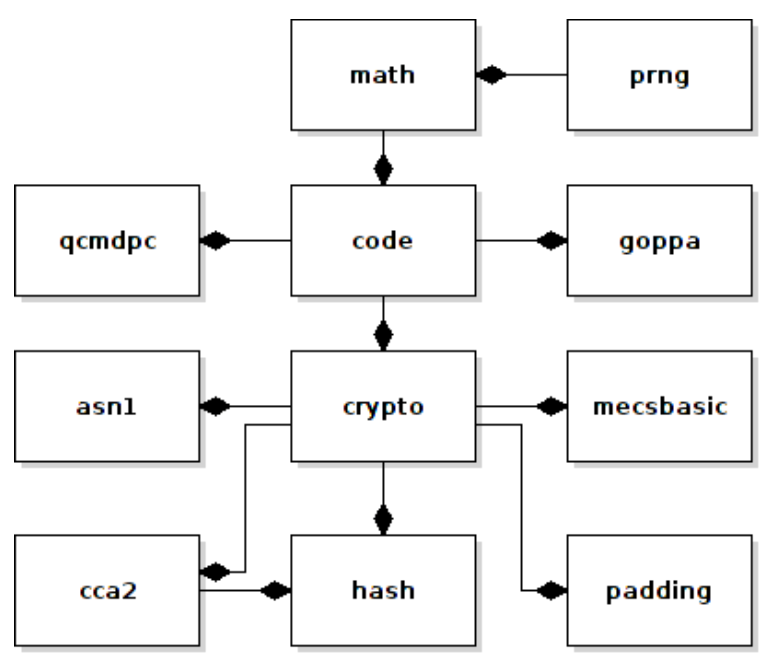
\includegraphics[width=10cm]{img/architecture.png}
	\caption{Modular architecture of Bitpunch.}
	\label{architecture}
\end{figure}

\begin{itemize}
	\item asn1 - provides import/export of keys using libtasn1,
	code - provides implementation of used codes (Goppa, QC-MDPC [reff]),
	\item crypto: 
		\begin{itemize}
			\item cca2 - implementation of CCA2 conversions,
			\item hash - implemented hash from PolarSSL 
			\item mecsbasic - implementation of basic McElice PKC,
		\item padding - implementation of padding,
		\end{itemize} 
	\item math - provides arithmetic functions over $Gf(2^m)$, etc.
	\item prng - API for a pseudo random generator
\end{itemize} 
As we consider the architecture to be ....TODO: treba popisat, ze libka je dobre rozdelena na moduly a nebudeme to menit

\subsubsection{CCA conversions}
In this section, we discuss CCA conversions, which should provide indistinguishability under
adaptive chosen-ciphertext attacks.

The original version of MECS is not secure in theoretical way. In practice, a PKC can be considered secure to use if it provides IND-CCA security. The current version of Bitpunch includes a version of Pointcheval conversion. An input of the conversion is a plaintext. 
 
\paragraph{Variant of Pointcheval CCA2 conversion} % (fold)
\label{par:cca2_pointcheval_konverzia}
\begin{algorithm}[H]
	\caption{The Pointcheval CCA2 conversion}
	\label{mecs_kgen}
	\begin{enumerate}
	\item An input of MECS is $\widehat{m} = r_1 || hash(m || r_2)$, $r_1$ is a random bit vector with lenght $k - l$ and output of hash function is indistinguishable from random $l$-bit vector,
	\item A ciphertext consists of $(c_1, c_2, c_3) = (\widehat{m}\widehat{G} + e, hash(r_1) + m, hash(e) + r_2)$.
	\end{enumerate}
\end{algorithm}

This version of Pointecheval conversion is susceptible to the following attack.
TODO: treba dopisat utok


\noindent As it was discussed at [Komara and Imai], the original version of MECS is susceptible to partially-known plaintext,
related plaintext, reaction attacks and also does not provide security against malleability. However, Kobara and Imai presented two slightly different CCA conversion of MECS, which are considered to be secure against already mentioned attacks. These conversions require the use of random oracles (hash functions) [2] to randomize the input and break relations of
the plaintext and ciphertext. Unfortunately, conversions cause an overhand since some redundant data are necessary.
As is depicted on the figure [referencie], an algorithm for encryption is straightforward and can be described as follow: The input of this process is a public key $(G',t)$, a message $m$ and constant $Const$, which sum of its $(m||Const)$ length. The output of encryption is a ciphertext. The decryption process is described respectively by following algorithms.

\begin{algorithm}[H]
	\caption{Kobara-Imai CCA2 gamma conversion - encryption}
	\label{kobara-enc}
	\begin{enumerate}
		\item Let $m$ be a message, a constant $Const$ and a random $r$-bit number $Rand$,
		\item Calculate $y_1 = Prng(Rand) + (m || Const)$,
		\item Calculate $y_2 = HASH(y_1) + Rand$,
		\item Let $y_1 = y_1' || y_4 || y_3$,
		\item Let $y_5 = y_2 || y_1'$, 
		\item Encode error vector $e = CONV(y_4)$,
		\item Encrypt $y_3$ using MECS such that $y_6 = MECS_{enc}(e, y_3) = y_3G' + CONV(y_4)$, 
		\item A ciphertext is $c = y_5 || y_6$.
	\end{enumerate}
\end{algorithm}


\begin{algorithm}[H]
	\caption{Kobara-Imai CCA2 gamma conversion - decryption}
	\label{kobara-dec}
	\begin{enumerate}
		\item Let $c$ be the received message, $c = y_5 || y_6$ and the constant $Const$,
		\item Decrypt $y_6$ using MECS $(e, y_3) = MECS_{dec}(y_6)$, where $e$ is the error vector,
		\item Decode $y_4 = CONV^{-1}(e)$,
		\item Let $y_5 = y_2 || y_1'$, we reconstruct $y_2$ and $y_1$ such that $y_1 = y_1' || y_4 || y_3$,
		\item Calculate $Rand = y_2 + HASH(y_1)$,
		\item Calculate $(m||Const') = PRNG(Rand) + y_1$,
		\item If $Const'$ is equal to $Const$, the integrity of message is not corrupted,
		\item The plaintext is $m$.
	\end{enumerate}
\end{algorithm}

  
 \begin{figure}[!htbp]
 	\centering
 	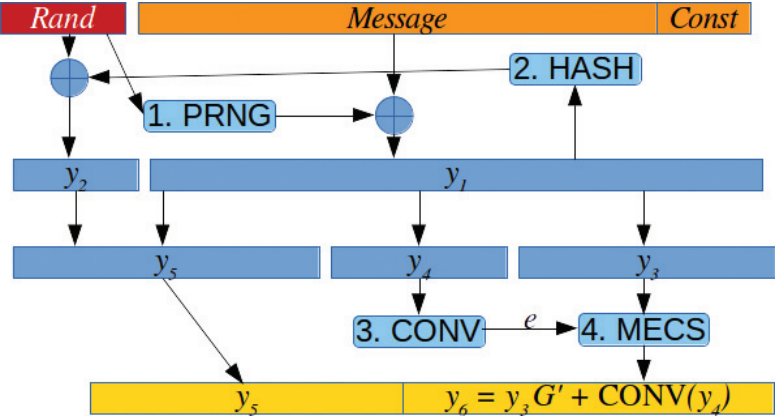
\includegraphics[width=12cm]{img/kobaraImai.png}
 	\caption{An illustration of the Kobara-Imai CCA-2 secure conversion of MECS.}
 	\label{kobara-imai}
 \end{figure}
 
\newpage
\label{kobara imai}
\begin{itemize}
	\item $Rand$ is a random session key (with size given by the required security,
	level for symmetric encryption).
	\item $PRNG$ is a cryptographically secure pseudorandom generator (can be
	a symmetric encryption algorithm in practice).
	\item $Const$ is a public constant (with size given by the required security level
	for authentication).,
	\item $HASH$ is a cryptographically secure hash function.
	\item $CONV$ is a bijection function, which converts an integer into the corresponding error vector.
	\item $MECS$ is a standard MECS routine (with e as an additional input).
\end{itemize}

\newpage


\section{Our contribution}


\begin{algorithm}
\lstset{
    language=C,
    basicstyle=\small\sffamily,
    frame=none,
    numbers=left,
    xleftmargin=5.0ex,
    numberstyle=\tiny,
    stepnumber=1,
    showstringspaces=false,
    keywordstyle=\color{blue}\bfseries
    }
\lstset{emph={%  Adjust any special keywords
    printf%
    },emphstyle={\color[rgb]{1,0,0}\bfseries}%
}%
\begin{lstlisting}
/* Hello World program */

#include<stdio.h>

struct cpu_info {
    long unsigned utime, ntime, stime, itime;
    long unsigned iowtime, irqtime, sirqtime;
};

main()
{
    printf("Hello World");
}\end{lstlisting}
 \caption{algoritmu}
 \label{euclid}
\end{algorithm}